\documentclass[12pt]{article}

%**********************************************
%* Add additional packages as needed

\usepackage{url,amsmath,setspace,amssymb}
\usepackage{listings}

\usepackage{tcolorbox}
\usepackage{tikz}
\usepackage{xcolor}


\usepackage{color}
\def\R{\color{red}}
\def\B{\color{blue}}

\usepackage{listings}
\usepackage{caption}
\newcommand{\inlinecode}{\texttt}



%**********************************************
%* Please replace this with your name and your AAU student number
\newcommand{\studentname}{Lorenzo Zanolin}
\newcommand{\studentnumber}{12245822}



%**********************************************
%* Some more or less useful stuff, add custom stuff as needed

\lstnewenvironment{myalgorithm}[1][] %defines the algorithm listing environment
{
   % \captionsetup{labelformat=algocaption,labelsep=colon}
    \lstset{ %this is the stype
        mathescape=true,
        frame=none,
        numbers=none,
        basicstyle=\normalsize,
        keywordstyle=\color{black}\bfseries\em,
        keywords={,input, output, return, datatype, function, in, if, else, foreach, while, begin, end, },
        numbers=left,
        xleftmargin=.04\textwidth,
        #1 % this is to add specific settings to an usage of this environment (for instance, the caption and referable label)
    }
}
{}


\newtcolorbox{alert}[1]{
colback=red!5!white, colframe=red!75!white,fonttitle=\bfseries, title = #1}

\newtcolorbox{commentbox}[1]{
colback=black!5!white, colframe=black!75!white,fonttitle=\bfseries, title = #1}



%**********************************************
%* Leave the page configuration as is
\setlength{\oddsidemargin}{.25in}
\setlength{\evensidemargin}{.25in}
\setlength{\textwidth}{6.25in}
\setlength{\topmargin}{-0.4in}
\setlength{\textheight}{8.5in}

\newcommand{\heading}[5]{
\renewcommand{\thepage}{#1-\arabic{page}}
\noindent
\begin{center}
	\framebox[\textwidth]{
	\begin{minipage}{0.9\textwidth} \onehalfspacing
	{\bf 622.755 -- \unitname} \hfill #2

	{\centering \Large #5

	}\medskip
	{#3 \hfill #4}
	\end{minipage}
}
\end{center}
}

\newcommand{\unitname}{Introduction to Cybersecurity}
\newcommand{\maxpages}{5}
\newcommand{\handout}[3]{\heading{#1}{#2}{\studentname}{\studentnumber}{#3}}
\bibliographystyle{plain}
%**********************************************
%* The document starts here
\begin{document}
\handout{\maxpages}{Summer Term, 2022/23}{Project Write Up}


\section{Outline}
The report is organized as follows: Section  \ref{sec:yao} offers an overview of Yao's protocol, including some insights of my implementation of the Secure Multiparty Computation (SMPC) adder \cite{smpc}. In Section \ref{sec:world}, I present a practical application of my implementation in real-world scenarios. Section \ref{sec:sel} delves into an analysis of the social, ethical, and legal considerations associated with this implementation. Finally, Section \ref{sec:end} provides a comprehensive summary of the entire report, encapsulating its contents.

\section{Yao's protocol}\label{sec:yao}
This project covers the Yao's protocol\cite{yao}; more precisely the \textit{Secure Multi-Party Computation}. This protocol allows two parties, Alice who knows x and Bob who knows y, to compute jointly the value of $f(x, y)$ in a way that does not reveal to each side more information than can be deduced from $f(x, y)$\cite{ot}.
In this scenario Alice is the garbler, while Bob is the evaluator. Another important role is the use of the \textit{OT}\cite{ot}, which is responsible to let Bob knows his encrypted input. An example of functioning is represented in figure \ref{steps}.

\begin{figure}[h]
    \makebox[\textwidth][c]{
    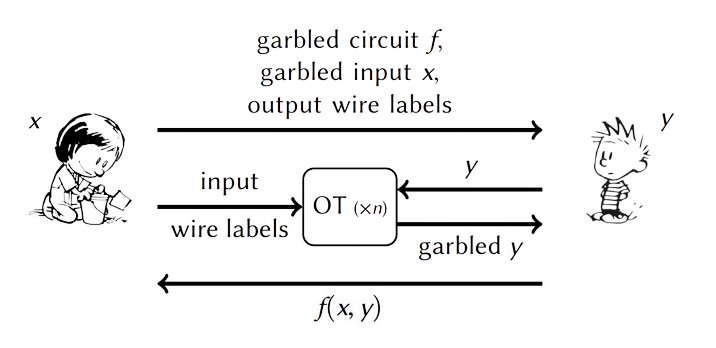
\includegraphics[width=1.1\linewidth]{../src/images/steps.png}}
    \caption{Steps of the SMPC}\label{steps}
\end{figure}

\footnote{\ref{steps} was taken from \url{https://web.engr.oregonstate.edu/~rosulekm/cryptabit/1-overview.pdf}
\ref{half} was taken from \url{https://upload.wikimedia.org/wikipedia/commons/1/14/Half-adder.svg}\\ 
\ref{full} was taken from \url{https://upload.wikimedia.org/wikipedia/commons/a/a9/Full-adder.svg}.}
\vspace{2mm}
There are two principles that must be respected\cite{principles}: 
\begin{itemize}
    \item \textit{privacy}: nothing is learned from the protocol other than the output;
    \item \textit{correctness}: the output is distributed according to the prescribed functionality.
\end{itemize}

The request was to implement a program for which two user can sum up their set of values without sharing them with the opposing party; in this case we decided to create a 8-bit adder circuit.
The circuit uses 7 full adders, 1 half adder and 1 if-then-else, represented in figures \ref{half} \ref{full} \ref{overflow}, concatenated together; the implementation of the entire circuit is represented in figure \ref{circuit}.
In this implementation, as you can read in my full review at \url{https://github.com/lorenzozanolin/garbledCircuit}\label{zanoGit}, \textit{privacy} is respected since neither Alice or Bob can understand the set of the other. The same holds for the \textit{correctness}: assuming that both actors behave always honestly, the result obtained through Yao's protocol is guaranteed to be the same as that obtained through a standard computation, and this is verified by a procedure inside the program.

\begin{figure}[!htb]
    \begin{center}
        \begin{minipage}{0.4\textwidth}
            \centering
            
\includegraphics[width=.7\linewidth]{../src/images/Half_adder.png}
            \caption{Half Adder}\label{half}
        \end{minipage}
        \hfill
        \begin{minipage}{0.4\textwidth}
            \centering
            
\includegraphics[width=.8\linewidth]{../src/images/Full-adder.png}
            \caption{Full Adder}\label{full}
        \end{minipage}
        \hfill
        \begin{minipage}{0.45\textwidth}
            \centering
            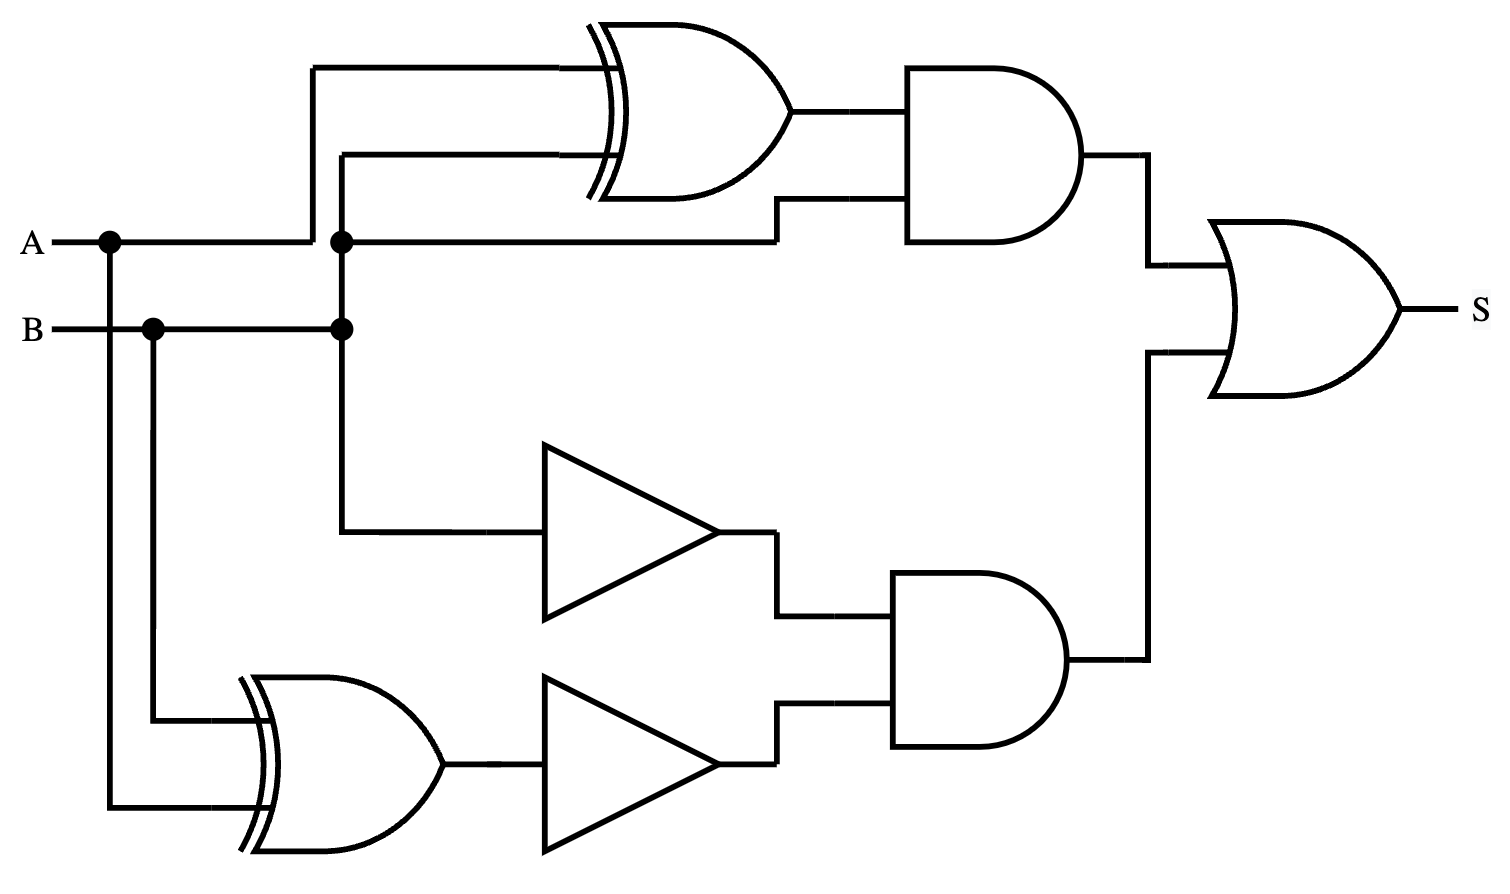
\includegraphics[width=1\linewidth]{../src/images/overflow.png}
            \caption{If then else}\label{overflow}
        \end{minipage}
    \end{center}
\end{figure}
\begin{figure}[!h]
    %\centering
    \makebox[\textwidth][c]{
    
\includegraphics[width=1.2\linewidth]{../src/images/Circuit.png}
    }
    \caption{8-bit Adder}\label{circuit}
\end{figure}

\section{Real word application}\label{sec:world}
%manca esempio generico
Secure multiparty computation protocols permit to compliantly, securely, and privately compute on distributed data without ever exposing or moving it. It permits parties to collaborate without compromising sensitive information to each other or third parties, enhancing trust and minimizing the episodes of data breaches. An important field where privacy is crucial is \textit{healthcare}. Medical institutions frequently require access to patient data from other healthcare providers to furnish better patient care; this informations must be kept private \cite{application}. SMPC is useful because it allows to perform a joint function, such as a \textit{statistical analysis}, on patient data while keeping it private. An example can be found in the paper \cite{healthcare}, in which it is shown how Yao's garbled circuit is used to compute how many patients from different institutions have high Charlson index or have visited an ED for at least 4 times within a year.
\subsection{Average salary calculator}
In the \textit{sum} case, an example could be the following: imagine you are an employee in a corporation and you want to know the average salary without revealing to anyone your income. In this scenario you can the use the \textit{SMPC} protocol to get everyone's data and compute the sum; then you can proceed calculating the mean. 
As example, think of a big corporation with multiple locations. We have four employees, respectively Alice, Bob, Eve and Charlie; they work in two different locations and they want to compute the average salary among them. In my implementation, there are two parties (that represent each one a single location) and both of them have a pair of integers that represent the salary. Thus, once the \inlinecode{main.py} is called, the sum of the sets is computed; now the final operation is to divide the result by the number of participants, to obtain the average.
In this example no one can understand values of other employees, thus \textit{privacy} is respected; same holds for the \textit{correctness} since the result obtained through Yao's protocol is guaranteed to be the same as that obtained through a standard computation. 
\section{Ethical, Legal and Social aspects}\label{sec:sel}
\subsection{Ethical considerations}
SMPC is useful for protecting user data and guaranteeing their anonymity, but at the same time it is important that this whole process does not lead to disadvantageous situations for some of the parties involved. Suppose we examine statistical surveys, where calculations are made to determine various metrics, such as the average salary of a particular group. It is common for such surveys to encounter unbalanced data, where certain subsets of data have significantly different properties than the others. Take as example a scenario where a company has multiple locations across the globe, where employees in less developed regions earn far less than their counterparts in more prosperous countries. In such a case, if the number of employees in the more prosperous regions is significantly greater than those in the lower-paid regions, the mean salary calculation could potentially be biased, leading to unreliable results. The problem here is intrinsic to the operation itself, SMPC is not really the guilty part; to overcome it, it should exist a control that checks whether the variation $\Delta$ of the inputs is below a predefined threshold.

\subsection{Legal considerations}
It's important that all the computations done must preserve confidentiality, let us analyze the 8-bit adder case. By construction of my solution, all inputs (sensible data) are encrypted using \textit{AES-CBC} as encryption scheme; thus all data that flows is encrypted. By definition, encryption is used to assure confidentiality. To delve into further details, we can refer to the \textit{General Data Protection Regulation} (GDPR). This regulation provides comprehensive data protection measures and imposes additional responsibilities on organisations involved in the collection and processing of such data. These guidelines ensure that appropriate security measures are implemented to protect personal data from unauthorised access, loss, or misuse. Some individuals or organisations may be hesitant to share their data, even in a secure and privacy-preserving manner, due to concerns about privacy breaches. There could be a need for clear communication and education (on how this technique works) to address these concerns and build confidence in the technology.

\subsection{Social considerations}
A significant social consideration when it comes to utilising secure multiparty computation (MPC) is the potential impact on trust and collaboration among participating parties. While MPC offers the advantage of secure computation without exposing sensitive inputs, it becomes crucial to address the issue of potential dishonest behavior among participants, as it could lead to unreliable results. In some cases, economic interests may come into play, where inputs are intentionally biased to manipulate the outcome; the challenge lies in identifying and addressing such situations since all data is encrypted, making it difficult to detect any manipulation or biased inputs. Finding ways to ensure the integrity of participants and establishing mechanisms for accountability become crucial aspects to consider in order to maintain the trustworthiness and reliability of MPC in practice. 
\section{Final considerations}\label{sec:end}
In conclusion, in this paper we briefly presented the Yao's Secure computation analysing an implementation of it. We further explored the practical applications of this technology in real-world scenarios, highlighting its significant potential. However, it is essential to pay attention when utilising this technology, as emphasised in Section \ref{sec:sel}. Due to the encryption of all information used, once the computation is performed, the data cannot be reversed; therefore, careful attention must be taken during the process of selection of inputs to ensure accurate and reliable results.
\bibliography{thud}
\end{document}



